\textbf{1. Everyday examples of waves.} Sound traveling through air, ripples spreading across water, light from a lamp, a pulse moving along a rope, and seismic waves traveling through Earth are familiar examples. Radio and Wi-Fi signals are also electromagnetic waves.

\[\boxed{\begin{gathered}
\text{Sound, water ripples, light, rope pulses,}\\
\text{seismic waves, and radio signals.}
\end{gathered}}\qquad\text{(A.1.1)}\]

\textbf{2. Disturbance waves and continuous waves.} A disturbance wave begins with a localized change, such as a single pulse, and carries that profile through a medium. A continuous wave is produced when the source oscillates repeatedly, creating a sustained sequence of crests and troughs. The distinction concerns how the source moves over time; both types propagate through space.

\[\boxed{\begin{gathered}
\text{A disturbance is localized in time.}\\
\text{A continuous wave is sustained by repeated oscillation.}
\end{gathered}}\qquad\text{(A.1.2)}\]

\textbf{3. Wavespeed of a disturbance.} Wavespeed is the distance a recognizable point on the disturbance travels divided by the elapsed time. For the two profiles below, the pulse advances by $\Delta x$ during $\Delta t$, so its speed is $c=\Delta x/\Delta t$. For a right-moving pulse, $u(x,t)=F(x-ct)$ keeps the same shape because a fixed feature satisfies $x-ct=\text{constant}$.

\begin{figure}[H]
\centering
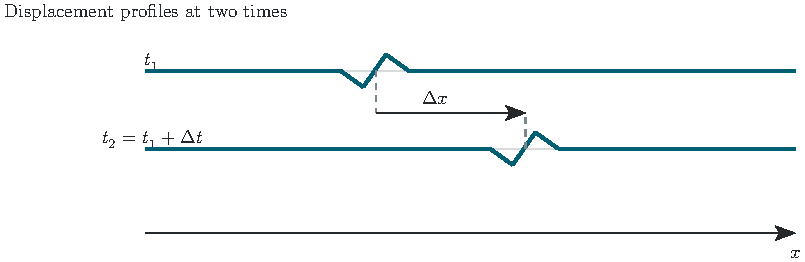
\includegraphics[width=0.82\linewidth]{figures/generated/solutions/A1-disturbance-speed.pdf}
\caption{A localized disturbance advances by $\Delta x$ during $\Delta t$.}
\end{figure}

\[\boxed{c=\frac{\Delta x}{\Delta t}}\qquad\text{(A.1.3)}\]

\noindent\begin{minipage}{\linewidth}\color{black}
\textbf{4. Equivalent disturbance-wave expressions.} For a right-traveling disturbance in a uniform medium with wavespeed $c$, let $F$ describe its profile and let $\ell>0$ be a reference length. Defining $G(\tau)=F(-c\tau)$ and $H(\xi)=F(\ell\xi)$ gives equivalent profiles written with a spatial, temporal, or dimensionless argument. Each expression therefore describes the same shape translating at speed $c$.

\[\boxed{u(x,t)=F(x-ct)=G\!\left(t-\frac{x}{c}\right)=H\!\left(\frac{x-ct}{\ell}\right)}\qquad\text{(A.1.4)}\]
\end{minipage}\par

\textbf{5. Interstate pileup.} A car pileup begins locally and spreads as vehicles encounter the slowdown. It is therefore a disturbance wave.

\[\boxed{\text{Disturbance wave (choice b).}}\qquad\text{(A.1.5)}\]

\textbf{6. Wavespeed of a continuous harmonic wave.} A harmonic wave has a sinusoidal profile that repeats as it propagates. Wavespeed is the speed of a fixed phase point, such as a crest. If that crest moves by $\Delta x$ during $\Delta t$, then $c=\Delta x/\Delta t$. For $u(x,t)=A\cos(\gamma x-\omega t+\phi)$, constant phase gives $\gamma x-\omega t+\phi=\text{constant}$ and hence $c=\omega/\gamma$.

\begin{figure}[H]
\centering
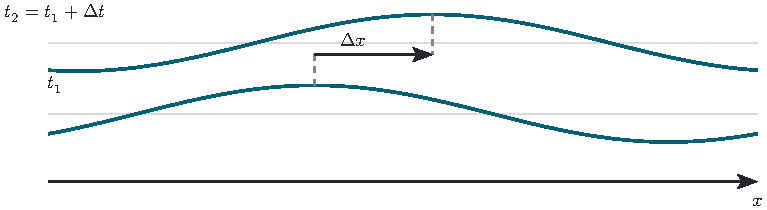
\includegraphics[width=0.82\linewidth]{figures/generated/solutions/A1-harmonic-speed.pdf}
\caption{A fixed phase point advances with the continuous harmonic profile.}
\end{figure}

\[\boxed{c=\frac{\Delta x}{\Delta t}=\frac{\omega}{\gamma}=f\lambda}\qquad\text{(A.1.6)}\]

\textbf{7. Wavelength and wavenumber.} Wavelength $\lambda$ is the spatial distance over which the harmonic profile completes one cycle, measured between adjacent points in the same phase, such as neighboring crests. Wavenumber $\gamma$ is the phase change per unit distance. Since one spatial cycle advances the phase by $2\pi$ radians over distance $\lambda$, the relationship is $\gamma=2\pi/\lambda$. Its SI unit is radians per meter, commonly written $\mathrm{rad/m}$.

\[\boxed{\gamma=\frac{2\pi}{\lambda},\qquad \lambda=\frac{2\pi}{\gamma}}\qquad\text{(A.1.7)}\]

\begin{figure}[H]
\centering
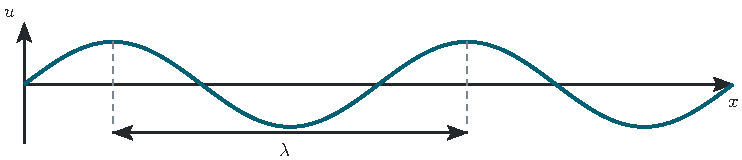
\includegraphics[width=0.82\linewidth]{figures/generated/solutions/A1-wavelength.pdf}
\caption{The wavelength spans one complete spatial cycle between matching phase points.}
\end{figure}

\begin{figure}[H]
\centering
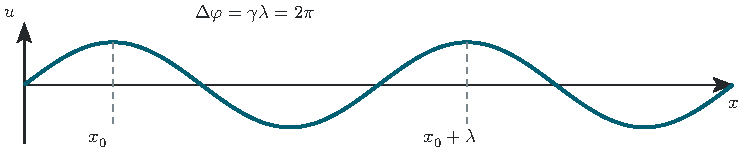
\includegraphics[width=0.82\linewidth]{figures/generated/solutions/A1-wavenumber.pdf}
\caption{Across one wavelength, the harmonic phase increases by $2\pi$ radians.}
\end{figure}

\textbf{8. Equivalent continuous harmonic-wave expressions.} A traveling harmonic wave can be written as a cosine with phase, a sine with an adjusted phase, or as the real part of a complex exponential. These forms describe the same oscillatory motion with suitable choices of amplitude and phase. Here $A$ is the amplitude, $\omega$ is angular frequency, $\gamma$ is wavenumber, and $\phi$ is phase.

\[\boxed{\begin{aligned}
u(x,t)&=A\cos(\gamma x-\omega t+\phi)\\
&=A\sin(\gamma x-\omega t+\phi+\tfrac{\pi}{2})\\
&=\operatorname{Re}\!\left\{A e^{i(\gamma x-\omega t+\phi)}\right\}
\end{aligned}}\qquad\text{(A.1.8)}\]

\textbf{9. What waves carry.} A wave transports energy through space or through a medium. In a mechanical wave, particles of the medium oscillate around their equilibrium positions; the wave does not carry the medium along as a net flow of matter.

\[\boxed{\text{Energy (choice b).}}\qquad\text{(A.1.9)}\]

\textbf{10. Graduate work. Particle-wave duality of light.} Light propagates and interferes as an electromagnetic wave, yet exchanges energy with matter in discrete photons. A photon of frequency $f$ carries energy $E=hf$, where $h$ is Planck's constant; for light in vacuum its momentum is $p=h/\lambda$. The photoelectric effect shows that energy transfer occurs in photon-sized packets, while interference and diffraction reveal wave behavior. These observations reveal complementary aspects of light. Its wave behavior governs propagation and interference, while photon events describe localized exchanges with detectors and matter.

\[\boxed{E=hf,\qquad p=\frac{h}{\lambda}}\qquad\text{(A.1.10)}\]
